\documentclass[12pt, titlepage]{article}
\usepackage[USenglish]{babel}
\usepackage[utf8]{inputenc}
\usepackage{amssymb, amsmath}
\usepackage{bm}
\usepackage{color}
\usepackage[unicode]{hyperref}
\usepackage{url}
\hypersetup{
    colorlinks,
    citecolor=blue,
    filecolor=blue,
    linkcolor=blue,
    urlcolor=blue
}
\usepackage{graphicx}
\usepackage{grffile}
\usepackage{listings}
\usepackage{float}

\def\sgn{\operatorname{sgn}}
\title{LinUCB vs HybridLinUCB}
\date{\today}
\author{Radek Bartyzal}

\begin{document}
\begin{titlepage}
    \centering
    \vfill
    {\bfseries\Huge
        LinUCB vs HybridLinUCB in recommender systems
    }    
    \vfill
        
    
        
    {\bfseries\Large 
    Author:\\
    Radek Bartyzal (bartyrad@fit.cvut.cz)\\
    }    
    \vskip1cm
 
    \vskip1cm
    \today

    
    \vfill
\end{titlepage}

%\tableofcontents
\pagebreak

\section{Introduction}\label{sec:intro}
The algorithms LinUCB and HybridLinUCB are both introduced in the article A Contextual-Bandit Approach to
Personalized News Article Recommendation published in 2012.

The authors decided to model personalized recommendation of news
articles as a contextual bandit problem, a principled approach in
which a learning algorithm sequentially selects articles to serve
users based on contextual information about the users and articles,
while simultaneously adapting its article-selection strategy.

\section{Theory}\label{sec:theory}
Both algorithms are based on upper confidence bound algorithm (UCB) that uses a smarter way to balance
exploration and exploitation than a simple $\epsilon-greedy$ strategy. 
Specifically, in trial $t$, these algorithms
estimate both the mean payoff $\mu_{t,a}$ of each arm $a$ as well
as a corresponding confidence interval $c_{t,a}$, so that $|\mu_{t,a} - \mu_a| <
c_{t,a}$ holds with high probability. They then select the arm that
achieves a highest upper confidence bound: $a_t =
arg max_a (\mu_{t,a} + c_{t,a})$. With appropriately defined confidence intervals,
it can be shown that such algorithms have a small total $T$-
trial regret that is only logarithmic in the total number of trials $T$,
which turns out to be optimal. 

\subsection{LinUCB with Disjoint Linear Models (LinUCB)}
We assume the expected payoff of an arm $a$ is linear in its d-dimensional feature $x_{t,a}$ with some unknown coefficient vector $\theta^*_a$, namely:

$$
E[r_{t,a}|x_{t,a}] = x^T_{t,a}\theta^*_a
$$

\begin{itemize}
\item $a$ = arm = action = item to be recommended = e.g. article
\item $t$ = trial = in this case user ID
\item $r_{t,a}$ = reward of action $a$ in trial $t$ 
\item $x_{t,a}$ = features describing \textbf{both} user and the selected article $a$ at trial $t$. If the features of a user are his ratings, they will change with time.
\item $\theta^*_a$ = an unknown coefficient vector specific to arm $a$
\end{itemize}

This model is called disjoint since the parameters are not shared among different arms.
The solution is reached by a simple ridge regression.

\begin{figure}[h]
 \centering
 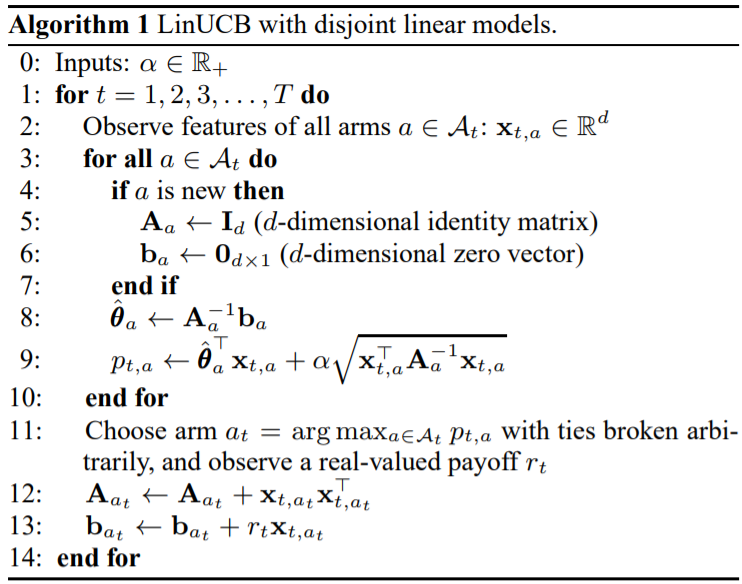
\includegraphics[scale=0.9]{img/LinUCB_alg}
 \caption{LinUCB algorithm with incrementally updating parameter matrices.}
 \label{fig:linUCB_alg}
\end{figure}

\subsection{LinUCB with Hybrid Linear Models (HybridLinUCB)}

In many applications, it is helpful to use features
that are shared by all arms, in addition to the arm-specific ones. For
example, in news article recommendation, a user may prefer only
articles about politics for which this provides a mechanism. Hence,
it is helpful to have features that have both shared and non-shared
components. Formally, we adopt the following hybrid model by
adding another linear term to the previous equation:

$$
E[r_{t,a}|x_{t,a}] = z^T_{t,a}\beta^* + x^T_{t,a}\theta^*_a 
$$

\begin{itemize}
\item $z_{t,a}$ = features of the current user/article combination
\item $\beta^*$ = an unknown coefficient vector common to all arms
\end{itemize}

\begin{figure}[h!]
 \centering
 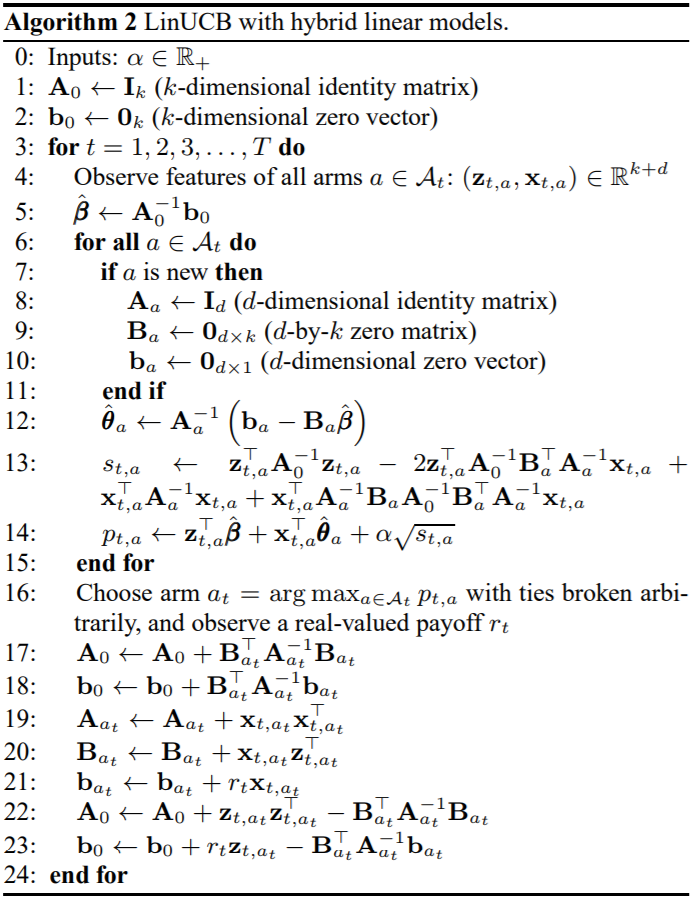
\includegraphics[scale=0.9]{img/HybridLinUCB_alg}
 \caption{HybridLinUCB algorithm with incrementally updating parameter matrices.}
 \label{fig:HybridlinUCB_alg}
\end{figure}


\section{Implementation}\label{sec:impl}



\section{Experiments}\label{sec:exp}

\begin{figure}[h]
 \centering
 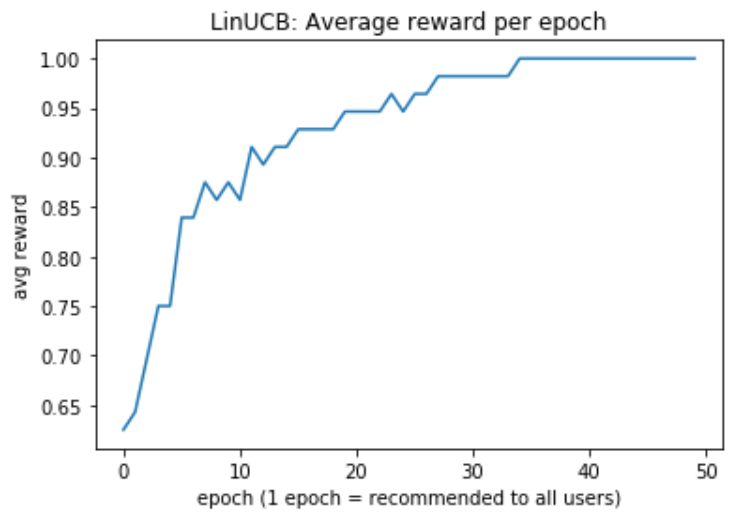
\includegraphics[width=\columnwidth]{img/LinUCB-100items-50epochs}
 \caption{LinUCB trained on 100 items and 56 users for 50 epochs.}
 \label{fig:linUCB-100it}
\end{figure}

\begin{figure}[h]
 \centering
 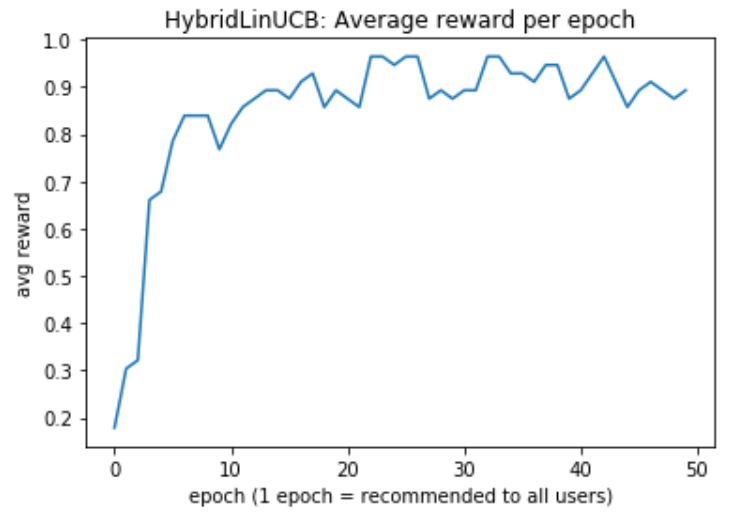
\includegraphics[width=\columnwidth]{img/HybridLinUCB-100items-50epochs}
 \caption{HybridLinUCB trained on 100 items and 56 users for 50 epochs.}
 \label{fig:HybridlinUCB-100it}
\end{figure}



\section{Conclusion}\label{sec:conclusion}


\begin{thebibliography}{0}

  \bibitem[1]{cit:ots} Li, Lihong, et al. "A contextual-bandit approach to personalized news article recommendation." Proceedings of the 19th international conference on World wide web. ACM, 2010. Accessible from: \url{https://arxiv.org/abs/1003.0146}
  
  \bibitem[2]{cit:ots} Project implementation at: \url{https://github.com/BartyzalRadek/contextual-bandits-recommender}
  

\end{thebibliography}


\end{document}